\documentclass[a4paper,10pt]{article}
\usepackage[utf8]{inputenc}
\usepackage[T1]{fontenc}
\usepackage{amsmath}

\usepackage{booktabs}

\usepackage{longtable}
\usepackage{tabu}

\usepackage{xspace}

\usepackage[sc]{mathpazo}
\linespread{1.05}

\newcommand*{\accgtitle}{Building a conveyor belt system editor \& simulator\xspace}
\newcommand*{\accgversion}{Draft, v2\xspace}

\usepackage[hidelinks]{hyperref}
\hypersetup{pdftitle={2IV05: \accgtitle}, pdfauthor={Thom Castermans \& Willem Sonke}}
\usepackage[format=hang]{caption}

\usepackage{graphicx}
\graphicspath{ {img/} }

\usepackage{geometry}

\usepackage[usenames,dvipsnames,svgnames,table]{xcolor}

\usepackage{changepage}

\usepackage[nottoc,notlof,notlot]{tocbibind} 
\tocotherhead{subsection}

\usepackage{subfig}

\renewcommand{\labelitemi}{$\bullet$}
\newcommand{\eo}[2]{#1\,/\,#2}

\begin{document}

\definecolor{accgblue}{RGB}{97,147,207}
\begin{adjustwidth}{0.05\textwidth}{0.05\textwidth}  
  \textcolor{accgblue}{\rule{0.9\textwidth}{0.8pt}}
  
  \begin{center}
    \large 2IV05 -- Additional component computer graphics\\
    \Large\textbf{\accgtitle}\\[10pt]
    \normalsize Thom Castermans \qquad Willem Sonke
  \end{center}
  
  \vspace{10pt}\noindent\footnotesize~~Eindhoven University of Technology\hfill\accgversion\ -- \today~~
  
  \vspace{-6pt}\noindent\textcolor{accgblue}{\rule{0.9\textwidth}{0.8pt}}
\end{adjustwidth}

\begin{abstract}
  \noindent This document is the second version of a report that will summarise the process of building an editor and simulator for conveyor belt systems. It also shows the resulting program.
\end{abstract}

\tableofcontents

\newgeometry{twoside}

\section{Introduction}
\label{sec:introduction}
In this report, we describe the program we created to simulate a system of conveyor belts that transport luggage items.

The system could potentially be used as a tool for modelling for example a luggage system at an airport. However, we have decided to make our application more like a game, since a real simulation system would be very difficult to make and furthermore require specialized domain knowledge about the system to simulate.

Before we started working on the project, we created a mock-up, as shown in Figure~\ref{fig:mockup}.

\begin{figure}
  \begin{center}
    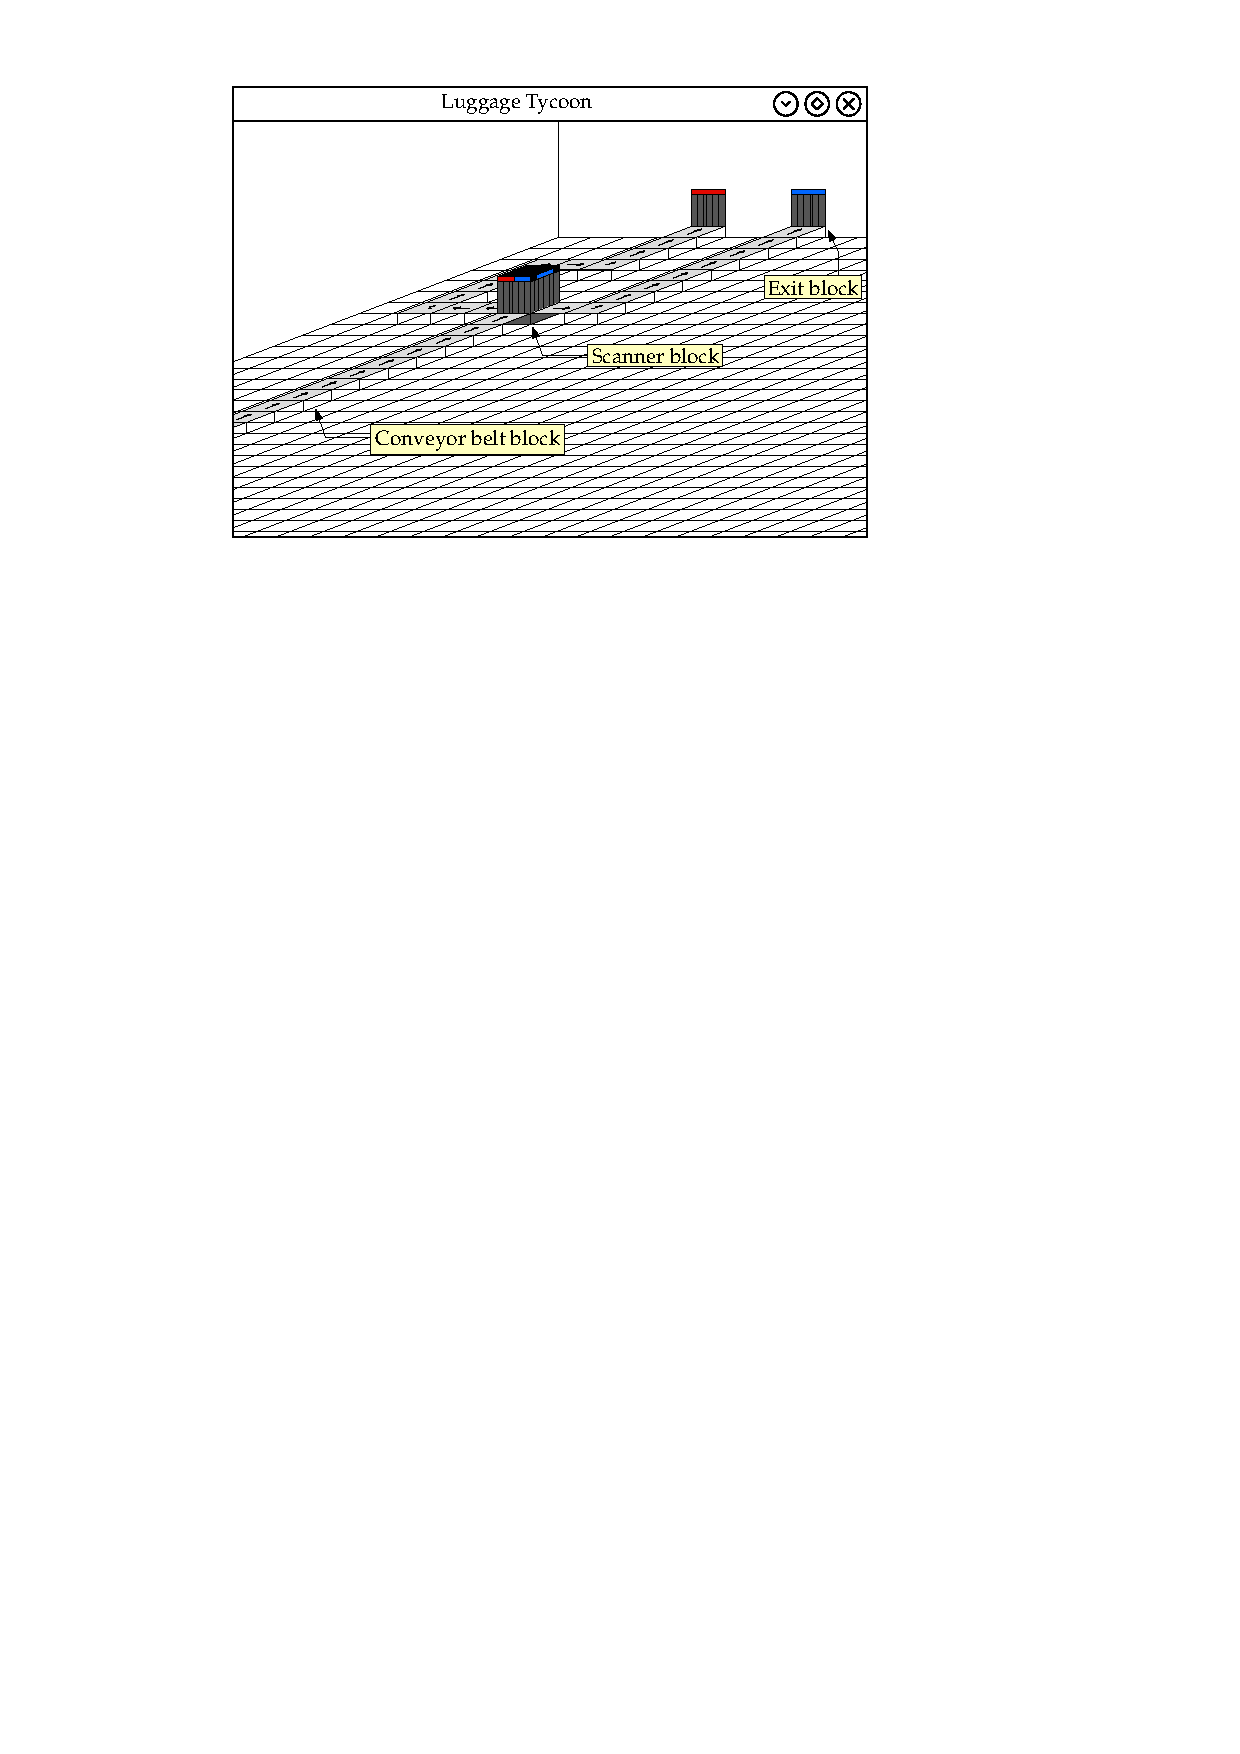
\includegraphics{mockup}
    \caption{A mock-up of the program we wanted to create.}
    \label{fig:mockup}
  \end{center}
\end{figure}


\section{Analysis}
\label{sec:analysis}
In this section, we divide the problem into subproblems, and analyse them separately.

We can divide the requirements into the two following subproblems.
\begin{itemize}
 \item \emph{The editor.} We need to show the conveyor belt system, and enable the user to edit it by adding new conveyor belts and removing them. This includes a GUI for the user to for example choose blocks.
 \item \emph{The simulator.} We need to simulate and show movement of luggage over the conveyor belts.
\end{itemize}
We can subdivide the editor again in several parts.
\begin{itemize}
 \item \emph{Viewing conveyor belts.} We need to show the conveyor belt system to the user in 3D.
 \item \emph{The interface.} We need to have an interface with which the user can choose different kinds of blocks, rotate them, and so on.
 \item \emph{Placing blocks.} Finally, the user needs to have a way to indicate where blocks should be placed or removed; therefore, we need to be able to convert 2D mouse clicks to the corresponding 3D location.
\end{itemize}

\subsection{Viewing}
\textbf{TO DO schetsen van de verschillende soorten banden en hoe ze eruit zien -- of dit in de vorige sectie misschien?}

\textbf{TO DO het aan elkaar tekenen van banden.}

\subsection{Interface}
\textbf{TO DO}

\subsection{Placing}
\textbf{@Thom: hier iets over dat lijn-in-cel-algoritme?}

\subsection{Simulation}

\section{Choices}
\label{sec:choices}
\textbf{TO DO}

\subsection{Simulating luggage movement in a conveyor belt system}
We initially implemented a simulation module ourselves, that was able to move luggage over the conveyor belts, but it did not support rotations. This means that luggage did not for example rotate when climbing an ascending conveyor belt or when it dropped of a belt. Furthermore the system was not really realistic, since we only used a very simple physics model. This meant that there was no collision detection between luggage items at all, and one piece of luggage could be placed inside another one.

After searching information about how to implement a more realistic physics system, we found out that it is extremely difficult to do so, and we decided to use an external library for the physics, named \emph{Bullet} (more accurately, a Java port of Bullet called \emph{JBullet}). Now we had to integrate JBullet in our application, which was not too difficult to do.

Initially, we had a little problem with getting the conveyor belts to actually move in JBullet. The belts were animated, but luggage would not move when it would fall on a conveyor belt. We found ways of simulating conveyor belts in Bullet, but unfortunately we were not able to use this since JBullet, the Java port we were using, was a couple of versions behind on Bullet. Finally, we found a way that worked in JBullet as well. Bullet has a notion of static objects. These are objects without mass that cannot (and will not) move. It is however possible to give these objects a linear and angular velocity, which results in dynamic objects hitting that static object taking over those velocities. This is precisely what we could use to simulate conveyor belts. We even managed to simulate curved conveyor belts realistically using a combination of a diagonal linear velocity and a non-zero angular velocity.

\section{Literature}
\label{sec:literature}
\textbf{TO DO}

\bibliographystyle{abbrv}
\tocsection
\bibliography{references}

\section{Results \& evaluation}
\label{sec:results}
\textit{The program is not done yet; when it is, we will expand this section.}

In this section, we will present the resulting program.

In Figure~\ref{fig:simulation}, a screenshot is shown of the program, while a simulation is running. \textbf{\ldots\ TO DO}

\begin{figure}
  \begin{center}
    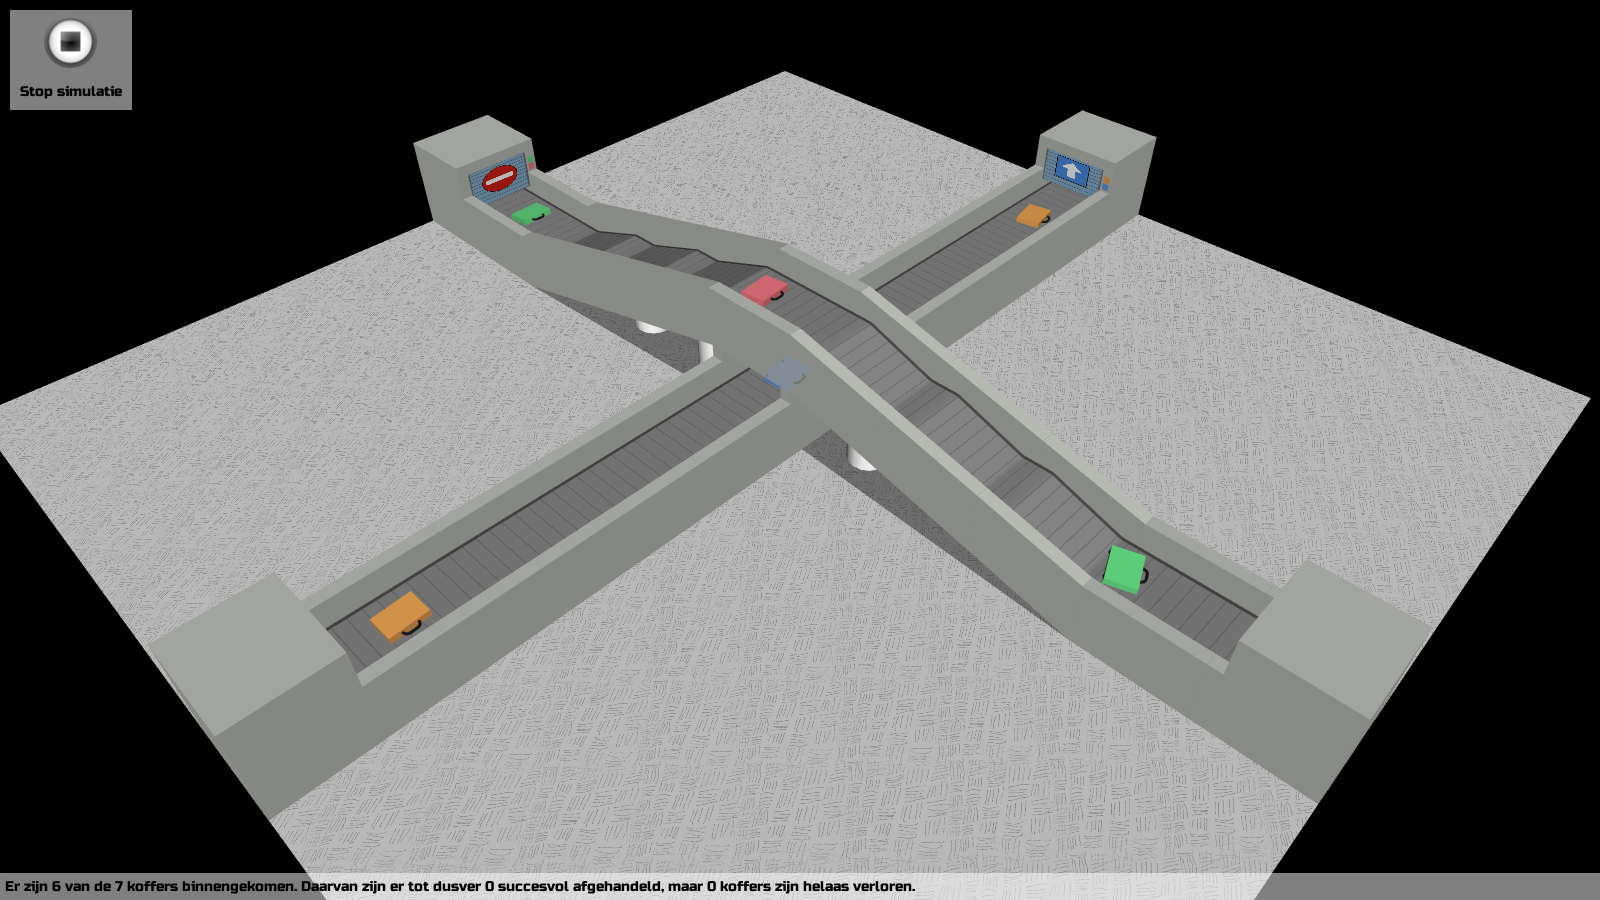
\includegraphics[width=\linewidth]{simulation}
    \caption{Screenshot of the program, showing a running simulation.}
    \label{fig:simulation}
  \end{center}
\end{figure}

\begin{figure}
  \begin{center}
    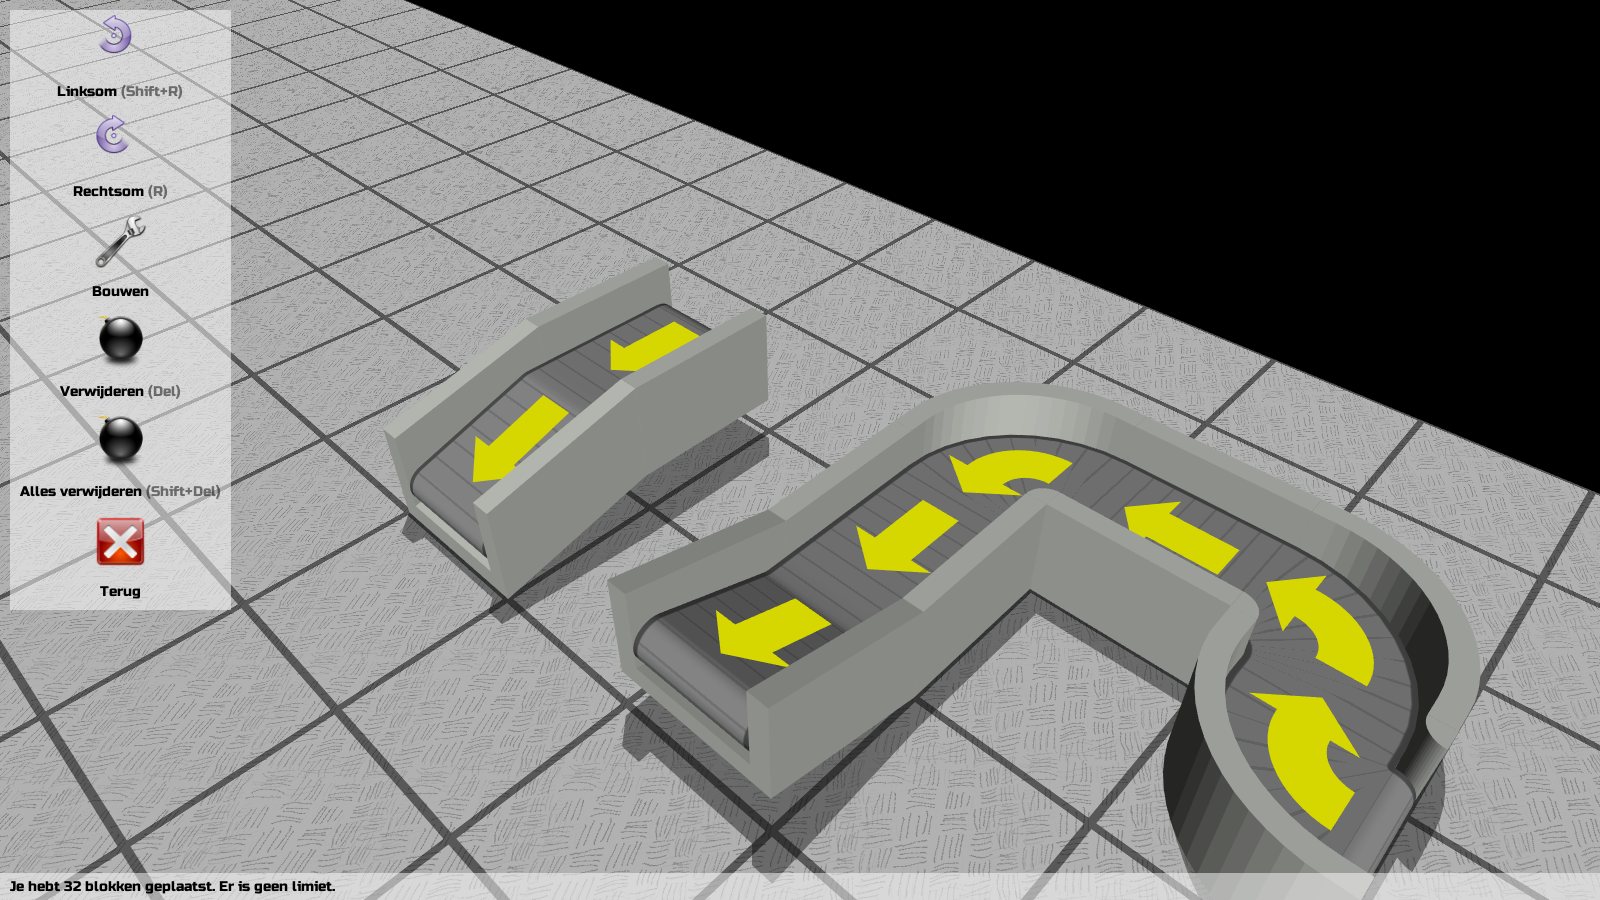
\includegraphics[width=0.7\linewidth]{drawing-together}
    \caption{Adjacent conveyor belts are drawn together as one large conveyor belt.}
    \label{fig:drawing-together}
  \end{center}
\end{figure}

\begin{figure}
  \begin{center}
    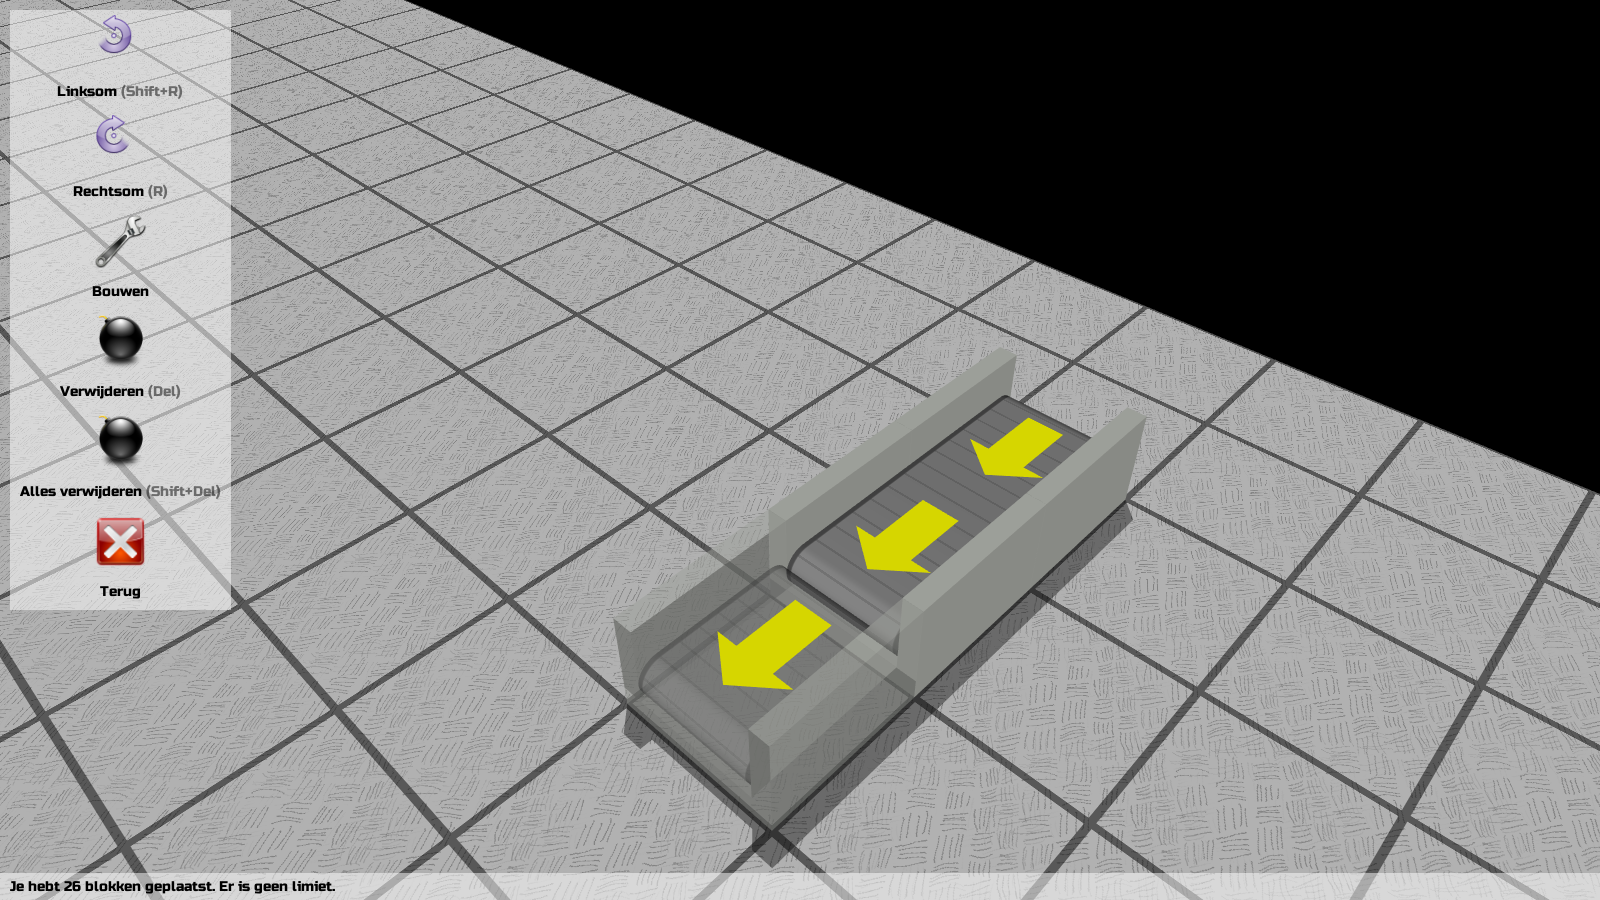
\includegraphics[height=0.3\linewidth]{shadow-block-1}
    \quad
    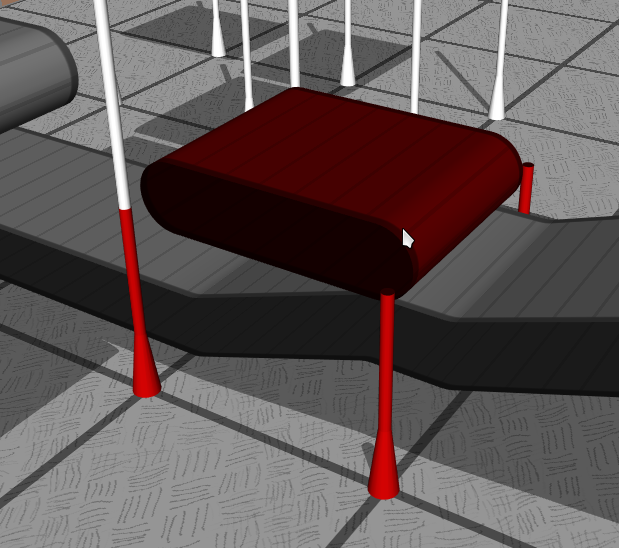
\includegraphics[height=0.3\linewidth]{shadow-block-2}
    \caption{Adding a new block. \textit{Left:} The block that is going to be added is shown as a ``ghost block'' under the cursor. \textit{Right:} If it is not possible to place the block on the indicated location, the ghost block becomes red to show this.}
    \label{fig:shadow-block}
  \end{center}
\end{figure}

\subsection{To be done}
There are quite some tasks that still need to be done.
\begin{itemize}
  \item Drawing more details for the conveyor belts.
  \item Drawing arrows to show the direction of conveyor belts in the building mode. More general, giving more clues to the user what to do (arrows, et cetera).
  \item Being able to choose an existing block to start from.
  \item Improvements to the graphical interface.
  \item Adding scanner blocks.
  \item Making the program more like a game, for example by adding levels and a scoring system.
  \item Being able to open and save conveyor belt systems.
\end{itemize}


\section{Conclusion}
\label{sec:conclusion}
\textit{In this section we will draw some conclusions when the program is ready. This includes: have we reached our goals, is the tool actually useful or fun to play with, et cetera.}

\section{Future work}
\label{sec:future-work}
We still have several ideas on how the resulting program could be improved. First of all, we have some ideas on how to improve the discoverability of features.
\begin{itemize}
 \item Users do not seem to notice how to drag a conveyor belt ``upwards'' to place a belt higher. This could be improved by giving a visual clue, for example an arrow.
 \item Another building mode to create long conveyor belts more easily.
\end{itemize}
Furthermore, there are some additional features that would make the game experience more interesting.
\begin{itemize}
 \item ``Scanners'' could be added that sort the luggage based on its color. This would make much more interesting levels possible.
 \item In the sandbox mode, the user should be able to place and remove the enter and exit points of luggage, and change its properties.
\end{itemize}


\end{document}
